\documentclass[../main]{subfiles}
\begin{document}

\chapter{非线性丙类功率放大器实验}%
\label{cha:非线性丙类功率放大器实验}

\section{实验目的}%
\label{sec:\arabic{chapter}实验目的}

\begin{enumerate}

	\item 了解丙类功率放大器的基本工作原理,掌握丙类放大器的调谐特性以及负载
		改变时的动态特性;

	\item 了解高频功率放大器丙类工作的物理过程以及当激励信号变化对功率放大器
		工作状态的影响;

	\item 比较甲类功率放大器与丙类功率放大器的特点、功率、效率。

\end{enumerate}

\section{基本原理}%
\label{sec:\arabic{chapter}基本原理}

非线性丙类功率放大器通常作为发射机末级功放以获得较大的输出功率和较高的效率。特点
:非线性丙类功率放大器通常用来放大窄带高频信号(信号的通带宽度只有其中心频率的1%
或更小),基极偏置为负值,电流导通角 ,为了不失真地放大信号,它的负载必须是LC谐振
回路。

电路原理图如图\ref{fig:非线性丙类功率放大器}所示,该实验电路由两级功率放大器组成
。其中$ Q_3 $(3DG12)、$ T_6 $组成甲类功率放大器,工作在线性放大状态,其中$
\mathrm{RA}_3 $、 $ R_{14} $、 $ R_{15} $组成静态偏置电阻,调节$ \mathrm{RA}_3 $
可改变放大器的增益。$ W_1 $为可调电阻,调节$ W_1 $可以改变输入信号幅度,$ Q_4 $
( 3DG12 )、$ T_4 $组成丙类功率放大器。$ R_{16} $为射极反馈电阻,$ T_4 $为谐振
回路,甲类功放的输出信号通过$ R_{13} $送到$ Q_4 $基极作为丙放的输入信号,此时只
有当甲放输出信号大于丙放管$ Q_4 $基极-射极间的负偏压值时,$ Q_4 $才导通工作。与
拨码开关相连的电阻为负载回路外接电阻,改变$ S_1 $拨码开关的位置可改变并联电阻值
,即改变回路$ Q $值。

\begin{figure}[htbp]
	\centering
	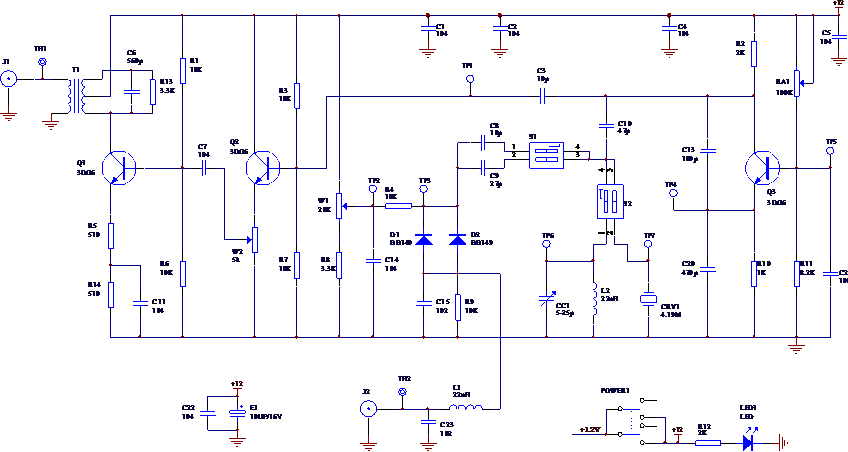
\includegraphics[width=0.8\linewidth]{circuit.png}
	\caption{非线性丙类功率放大器}
	\label{fig:非线性丙类功率放大器}
\end{figure}

\section{实验步骤}%
\label{sec:\arabic{chapter}实验步骤}

\subsection{测试调谐特性}%
\label{sub:测试调谐特性}

\footnote{做实验之前请将$ S_4 $开关拨下。}在前置放大电路出入$ J_3 $口处输入频率
\SI{10.7}{\MHz}($ V_\mathrm{p-p}\approx \SI{880}{\mV} $)的高频信号,调节$ W_1 $
和中周$ T_6 $,使$ \mathrm{TP}_6 $处信号的电压幅值为$ 3.2V $左右,$ S_1 $至$ S_3
$全部拨下,改变输入信号频率,从 \SI{9}{\MHz}$ \sim $\SI{15}{\MHz}(以
\SI{1}{\MHz}为步进)记录$ \mathrm{TP}_6 $处的输出电压值。

\subsection{测试负载特性}%
\label{sub:测试负载特性}

在前置放大电路中输入$ J_3 $口处输入频率\SI{10.7}{\MHz}($ V$ p-p $\approx
\SI{880}{\mV} $)左右的高频信号,调节$ W_1 $使$ \mathrm{TP}_6 $处信号约为
\SI{3.2}{\V}左右,调节中周使回路调谐(调谐标准:$ \mathrm{TH}_4 $处波形为对称双
峰)。

将负载电阻转换开关$ S_1 $依次从1—3拨动,用示波器观测相应的$ V_\mathrm{c} $值和$
V_\mathrm{e} $ 波形,分析负载对工作状态的影响。

\begin{table}[htbp]
	\centering
	\caption{测试负载特性}
	\label{tab:测试负载特性}
	\csvautobooktabular{tab/\arabic{chapter}/2.csv}
\end{table}

\begin{figure}[htbp]
	\centering
	\begin{subfigure}[htbp]{.45\linewidth}
		\centering
		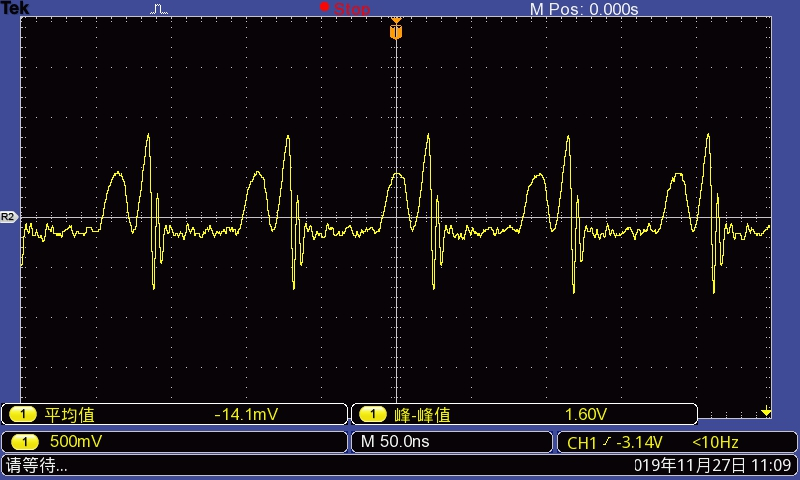
\includegraphics[width = \linewidth]{820.jpg}
		\caption{820欧姆}
		\label{fig:820欧姆}
	\end{subfigure}
	\quad
	\begin{subfigure}[htbp]{.45\linewidth}
		\centering
		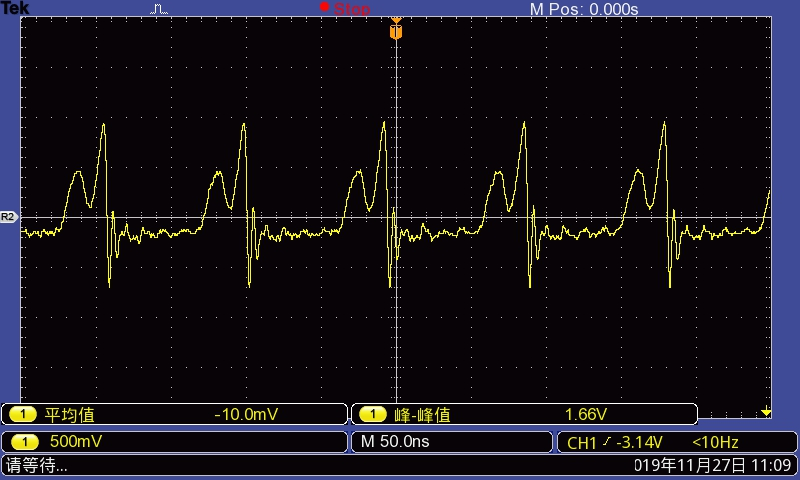
\includegraphics[width = \linewidth]{330.jpg}
		\caption{330欧姆}
		\label{fig:330欧姆}
	\end{subfigure}

	\begin{subfigure}[htbp]{.45\linewidth}
		\centering
		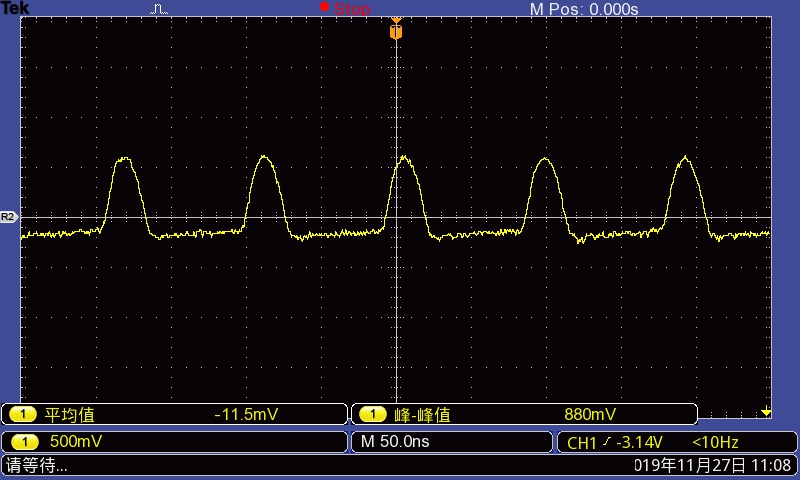
\includegraphics[width = \linewidth]{100.jpg}
		\caption{100欧姆}
		\label{fig:100欧姆}
	\end{subfigure}
	\quad
	\begin{subfigure}[htbp]{.45\linewidth}
		\centering
		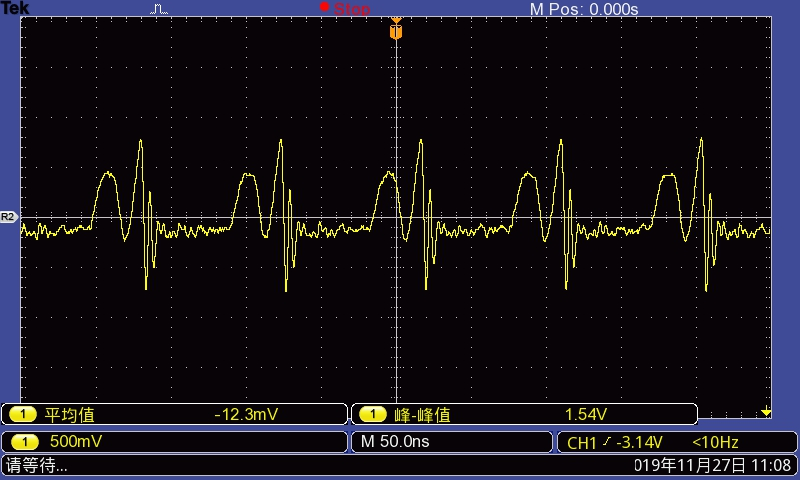
\includegraphics[width = \linewidth]{inf.jpg}
		\caption{无穷大欧姆}
		\label{fig:无穷大欧姆}
	\end{subfigure}
	\caption{测试负载特性}
	\label{fig:测试负载特性}
\end{figure}

\section{实验报告要求}%
\label{sec:\arabic{chapter}实验报告要求}

\begin{Exercise}

	整理实验数据,并填写表\ref{tab:测试负载特性}。

\end{Exercise}

\begin{Answer}

	实验数据见表\ref{tab:测试负载特性}。

\end{Answer}

\begin{Exercise}

	对实验参数和波形进行分析,说明输入激励电压、负载电阻对工作状态的影响。

\end{Exercise}

\begin{Answer}

	在丙类谐振功率放大器中, 根据晶体管工作是否进入饱和区,可将其分为欠压、
	临界和过压工作状态。临界状态输出功率最大,效率也较高,通常应选择在此状态
	工作。过压状态的特点是效率高、损耗小,并且输出电压受负载电阻 RL的影响小
	,近似为交流恒压源特性。欠压状态时电流受负载电阻 RL的影响小,近似为交流
	恒流源特性,但由于效率低、集电极损耗大,一般不选择在此状态工作。 丙类放
	大器的特点: 非线性丙类功率放大器通常用来放大窄带高频信号 ( 信号的通带宽
	度只有其中心频率的 1\%或更小 ) ,基极偏置为负值,电流导通角$ \theta <
	\ang{90;;} $,为了不失真地放大信号,它的负载必须是 LC 谐振回路。

\end{Answer}

\section{实验仪器}%
\label{sec:\arabic{chapter}实验仪器}

\begin{table}[htbp]
	\centering
	\caption{实验仪器}
	\label{tab:\arabic{chapter}实验仪器}
	\csvautobooktabular{tab/\arabic{chapter}/BOM.csv}
\end{table}

\end{document}

